%=========================Preamble====================================%
\documentclass[12pt] {article}
\usepackage{times}
\usepackage[margin=1in,bottom=1in,top=0.5in]{geometry}

\usepackage{graphicx}


\usepackage{float}
\usepackage{graphicx}
\usepackage{subfig}
\usepackage{wrapfig,lipsum}
\usepackage{amssymb}
\usepackage{nath}
\usepackage{amsfonts}


%=========================Doc====================================%
\begin{document}
\title{ECE 289A - An Introduction to Reinforcement Learning HW\#3}

\author{Ahmed H. Mahmoud}
\date{November, 2nd 2017} 
\maketitle
\section*{Q.1}
In this question, we regenerated plot in Figure 5.1 in the book. Figure \ref{fig:b} shows the regenerated plots.

\begin{figure}[!tbh]
\centering        
   \subfloat {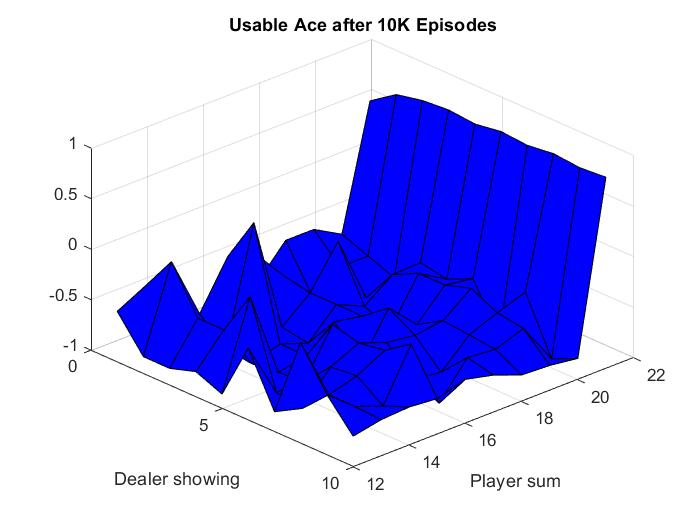
\includegraphics[width=0.49\textwidth]{../use10.jpg}}  
   \subfloat {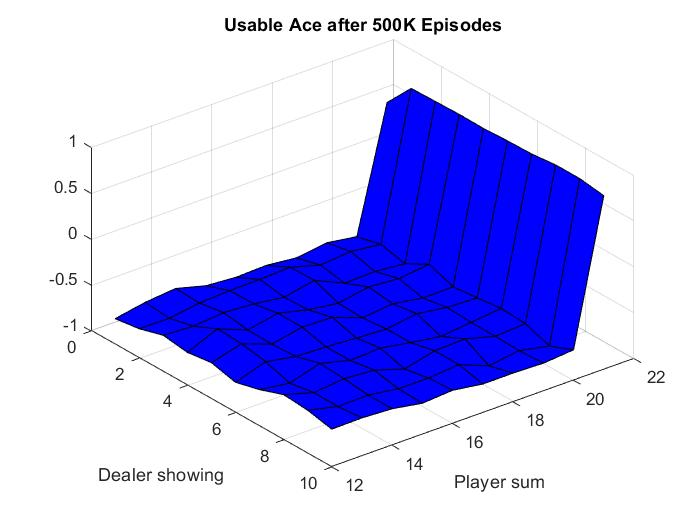
\includegraphics[width=0.49\textwidth]{../use50.jpg}}
        
   \subfloat {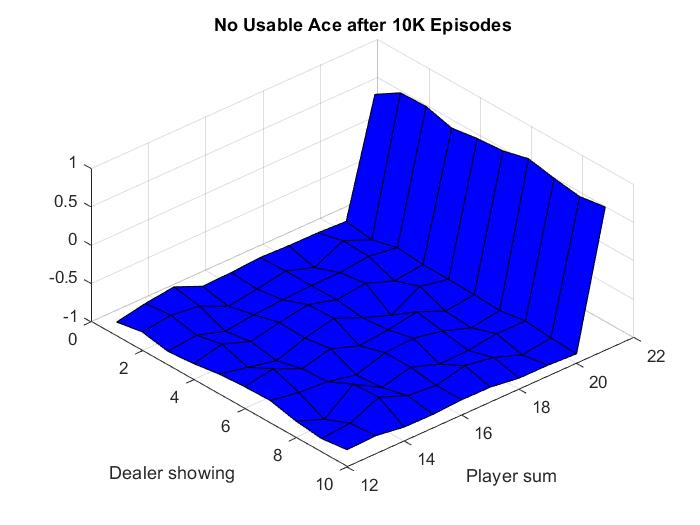
\includegraphics[width=0.49\textwidth]{../nouse10.jpg}}
   \subfloat {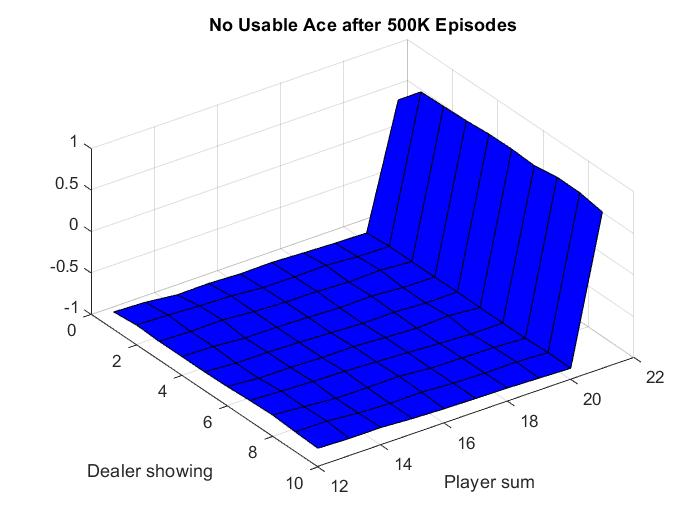
\includegraphics[width=0.49\textwidth]{../nouse50.jpg}}
      
   \caption{Approximate state-value functions for blackjack policy using Monte Carlo policy evaluation. }
   \label{fig:b}
\end{figure}

\section*{Q.2}
Here we regenerate Figure 5.4 from the book to compare the rate of convergence between weighted importance sampling and ordinary sampling. Figure \ref{fig:c} shows the regenerated plot.

\begin{figure}[!tbh]
\centering        
   \subfloat {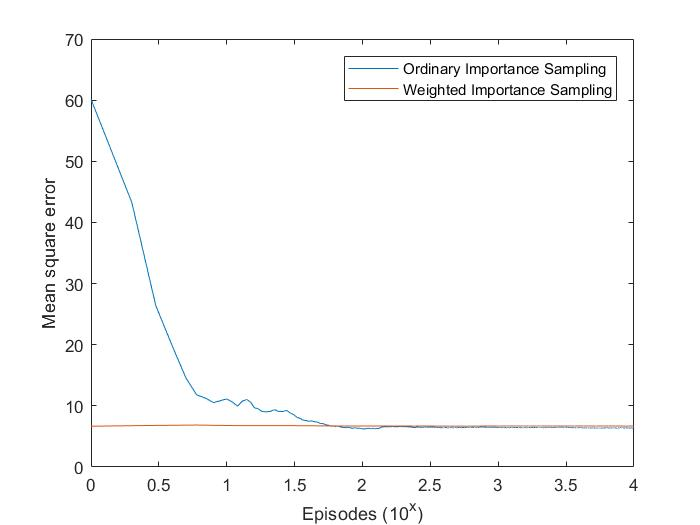
\includegraphics[width=0.7\textwidth]{../fig54.jpg}}        
   \caption{Weighted importance sampling produces lower error estimates of the value of a single blackjack state from off-policy episodes. }
   \label{fig:c}
\end{figure}

\end{document}
